\documentclass[12pt]{article}
\usepackage[english]{babel}
\usepackage[utf8]{inputenc}

%% Pointer to 'default' preamble, other reusable files
% pacakages and definitions

\usepackage{geometry}
\geometry{
	letterpaper, 
	portrait, 
	top=.75in,
	left=.8in,
	right=.75in,
	bottom=.5in		} 	% Page Margins
	
%% additional packages for nice things
\usepackage{amsmath} 	% for most math
\usepackage{commath} 	% for abs
\usepackage{lastpage}	% for page count
\usepackage{amssymb} 	% for therefore
\usepackage{graphicx} 	% for image handling
\usepackage{wrapfig} 	% wrap figures
\usepackage[none]{hyphenat} % for no hyphenations
\usepackage{array} 		% for >{} column characterisctis
\usepackage{physics} 	% for easier derivative \dv....
\usepackage{tikz} 		% for graphic@!
\usepackage{circuitikz} % for circuits!
\usetikzlibrary{arrows.meta} % for loads
\usepackage[thicklines]{cancel}	% for cancels
\usepackage{xcolor}		% for color cancels
\usepackage[per-mode=fraction]{siunitx} % for si units and num
\sisetup{group-separator = {,}, group-minimum-digits = 3} % additional si unit table functionality

\usepackage{fancyhdr} 	% for header
\usepackage{comment}	% for ability to comment out large sections
\usepackage{multicol}	% for multiple columns using multicols
\usepackage[framed,numbered]{matlab-prettifier} % matlab sytle listing
\usepackage{marvosym} 	% for boltsymbol lightning
\usepackage{pdflscape} 	% for various landscape pages in portrait docs.
%\usepackage{float}
\usepackage{fancyvrb}	% for Verbatim (a tab respecting verbatim)
\usepackage{enumitem}	% for [resume] functionality of enumerate
\usepackage{spreadtab} 	% for using formulas in tables}
\usepackage{numprint}	% for number format in spread tab
\usepackage{subcaption} % for subfigures with captions
\usepackage[normalem]{ulem} % for strike through sout

% for row colors in tables....
\usepackage{color, colortbl}
\definecolor{G1}{gray}{0.9}
\definecolor{G2}{rgb}{1,0.88,1}%{gray}{0.6}
\definecolor{G3}{rgb}{0.88,1,1}

% For table formatting
\usepackage{booktabs}
\renewcommand{\arraystretch}{1.2}
\usepackage{floatrow}
\floatsetup[table]{capposition=top} % put table captions on top of tables

% Caption formating footnotesize ~ 10 pt in a 12 pt document
\usepackage[font={small}]{caption}

%% package config 
\sisetup{output-exponent-marker=\ensuremath{\mathrm{E}}} % for engineer E
\renewcommand{\CancelColor}{\color{red}}	% for color cancels
\lstset{aboveskip=2pt,belowskip=2pt} % for more compact table
%\arraycolsep=1.4pt\def
\setlength{\parindent}{0cm} % Remove indentation from paragraphs
\setlength{\columnsep}{0.5cm}
\lstset{
	style      = Matlab-editor,
	basicstyle = \ttfamily\footnotesize, % if you want to use Courier - not really used?
}
\renewcommand*{\pd}[3][]{\ensuremath{\dfrac{\partial^{#1} #2}{\partial #3}}} % for larger pd fracs
\renewcommand{\real}[1]{\mathbb{R}\left\{ #1 \right\}}	% for REAL symbol
\newcommand{\imag}[1]{\mathbb{I}\left\{ #1 \right\}}	% for IMAG symbol
\definecolor{m}{rgb}{1,0,1}	% for MATLAB matching magenta
	
%% custom macros
\newcommand\numberthis{\addtocounter{equation}{1}\tag{\theequation}} % for simple \numberthis command

\newcommand{\equal}{=} % so circuitikz can have an = in the labels
\newcolumntype{L}[1]{>{\raggedright\let\newline\\\arraybackslash\hspace{0pt}}m{#1}}
\newcolumntype{C}[1]{>{\centering\let\newline\\\arraybackslash\hspace{0pt}}m{#1}}
\newcolumntype{R}[1]{>{\raggedleft\let\newline\\\arraybackslash\hspace{0pt}}m{#1}}

%% Header
\pagestyle{fancy} % for header stuffs
\fancyhf{}
% spacing
\headheight 29 pt
\headsep 6 pt
%%% custom commands for nicer units
\newcommand{\mw}{\ensuremath{\text{ MW}}}
\newcommand{\hz}{\ensuremath{\text{ Hz}}}
\newcommand{\pu}{\ensuremath{\text{ Pu}}}
\newcommand{\sbase}{\ensuremath{\text{S}_{\text{Base}}}}
\newcommand{\fbase}{\ensuremath{f_{\text{Base}}}}
\newcommand{\mbase}[1]{\ensuremath{\text{M}_{\text{Base}_{#1}}}}
\newcommand{\hsys}{\ensuremath{\text{ H}_{\text{sys}}}}


%% Header
\rhead{Thad Haines \\ Page \thepage\ of \pageref{LastPage}}
\chead{Six Machine Delay Scenario \\ 01-21-20}
\lhead{Research \\ }

%\usepackage{graphicx}
%\graphicspath{ {figures/} }
%\newcommand{\caseName}{ }

\begin{document}
\paragraph{Scenario: } 
Two area, six machine system loss of generation event. \\
Initially, $\approx$100 MW are being sent from Area 1 to Area 2 over the lines between bus 8 and 9.\\

% six machine system
\begin{figure}[!ht]
	\centering
	\footnotesize
	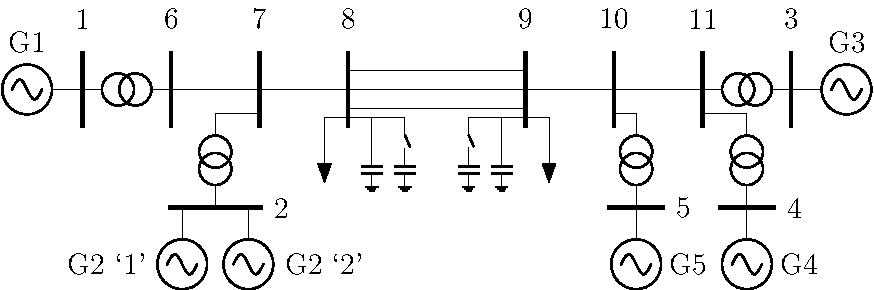
\includegraphics[width=.85\linewidth]{../../models/sixMachine/sixMachine}
	\caption{Six machine system.}
	\label{fig: six machine}
\end{figure}


Governed machines are: G1, G2 `1', G3, G4.\\
Governor time constants and generator inertia and MVA rating are identical for all machines.\\
No governor deadbands are used.\\
In cases that have AGC, PI filtered AGC signals are sent every 5 seconds to G1 and G3.\\

At t = 2, Generator 5 steps its mechanical power output $P_M$ down by 50 MW.\\

All system settings are the same in each test case unless noted otherwise.\\
% tgov delay

\begin{figure}[!ht]
	\centering
	\footnotesize
	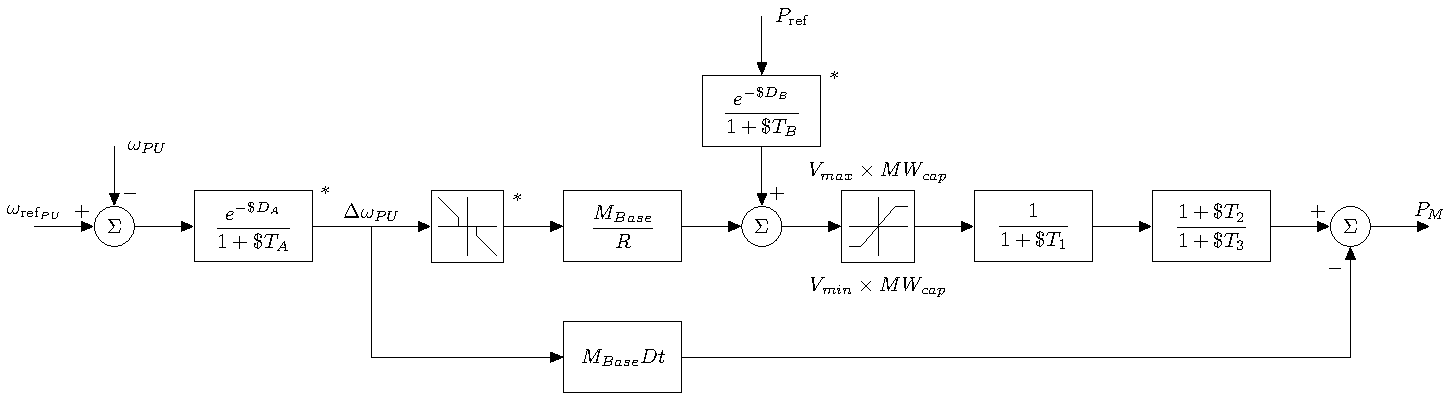
\includegraphics[width=.9\linewidth]{../../models/tgov1/tgov1DBdelay}
	\caption{Governor model with optional delays and deadbands indicated by a *.}
	\label{fig: modified tgov}
\end{figure}

For cases using delay, input $\Delta \omega_{PU}$ was delayed by 40 seconds and any changes to $P_{REF}$ were delayed by 10 seconds.

\paragraph{Results:} 
Delaying a governor response increased the frequency nadir and introduces a second frequency perturbance roughly 40 seconds after the first frequency event caused by the loss of generation.
Non-delayed governor action is required to eventually remove the frequency oscillations caused by the delayed governor response.
This is seen regardless of AGC action.
If there are equal amounts of delayed and non-delayed governor response, the system begins to oscillate.

\newcommand{\scrunch}{-.8em}
\newcommand{\caseName}{casename}

\newcommand{\resultPres}{%
\includegraphics[width=\linewidth]{figures/\caseName Freq}
\vspace{\scrunch}
\includegraphics[width=\linewidth]{figures/\caseName RACE}
\vspace{\scrunch}
\includegraphics[width=\linewidth]{figures/\caseName ValveTravel1}
\vspace{\scrunch}
\includegraphics[width=\linewidth]{figures/\caseName ValveTravel2}
\vspace{\scrunch}
\includegraphics[width=\linewidth]{figures/\caseName BranchMWflow8to9}
}

\pagebreak
\renewcommand{\caseName}{SixMachineDelayStep2}
\paragraph{No Delay, No AGC Results: } \ \\
50 MW generation drop - No AGC or delayed governor response.
\\
\resultPres

\pagebreak
\renewcommand{\caseName}{SixMachineDelayStep4}
\paragraph{Delay Governor, No AGC Results: } \ \\
Governor 1 has a 40 sec $\Delta \omega_{PU}$ delay.
\\
\resultPres

\pagebreak
\renewcommand{\caseName}{SixMachineDelayStep1}

\paragraph{AGC, No Delay Case Results:} \ \\
No Delay or filtering. AGC signals sent to Gen 1 and 3 every 5 seconds.
\\
\resultPres

\pagebreak
\renewcommand{\caseName}{SixMachineDelayStep3}
\paragraph{AGC with Delay Case Results: } \ \\
Generator 1 has a 40 sec $\Delta \omega_{PU}$ delay and a 10 sec $P_{ref}$ delay.
\\
\resultPres

\pagebreak
\renewcommand{\caseName}{SixMachineDelayStep5}
\paragraph{Equal  Delayed and Non-Delayed Governed Capacity: } \ \\
Governors are on Generator 1 and 3. Governor 1 in Area 1 is delayed. AGC is disabled.
\\
\resultPres


\end{document}